% !TEX root = ../main.tex

\section{研究区域与数据}

\subsection{研究区概况}

本文选取美国中西部玉米带内4个典型农业站点作为研究区，分别记为A、B、C和D。4个站点中，A、B位于爱荷华州，C位于印第安纳州，D位于伊利诺伊州，单个站点空间范围约为77~km~$\times$~77~km。该区域是美国重要的商品粮生产区，农田分布集中，种植类型以玉米和大豆为主，适合开展玉米大豆时空深度学习模型遥感识别及空间泛化能力分析。研究区空间位置如图1所示。

为分析研究区地表覆盖组成，本文采用美国农业部国家农业统计服务局发布的耕地数据层（Cropland Data Layer，CDL）数据。基于2021—2024年CDL数据统计结果，4个站点均以玉米和大豆为主要作物类型，两者面积之和均超过农作物总面积的95\%。本文将CDL原始类别重分类为玉米、大豆和其它3类，其中除玉米和大豆以外的农作物和非农作物地类都归并为"其它地物"，标记为其它。

\begin{figure}[tbp]
\centering
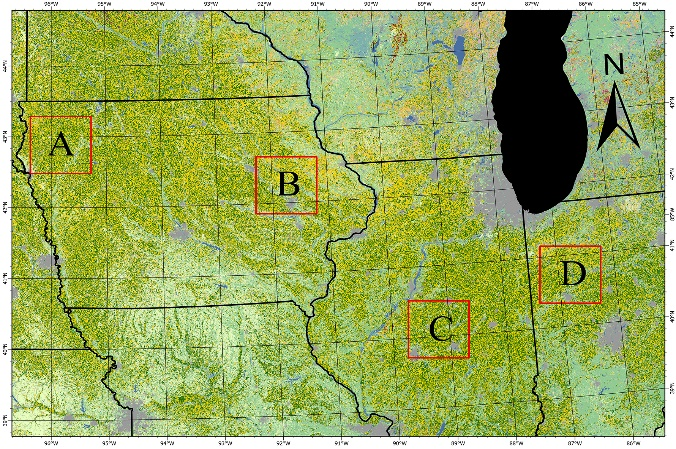
\includegraphics[width=\linewidth]{study_area/study_area.jpg}
\caption{研究区域4个站点分布图}
\label{fig:study_area}
\end{figure}

玉米和大豆物候信息来自美国农业部国家农业统计服务发布的作物进度报告（Crop Progress Report, CPR），其数据通过USDA NASS官网获取。结合CPR物候信息，本文将每年DOY~116—266作为主要观测窗口，该时间范围能够覆盖玉米和大豆的主要生育阶段。

\subsection{数据获取与预处理}

本文采用的多时相遥感数据源自美国国家航空航天局（NASA）地球数据科学系统提供的协同陆地卫星和哨兵2号数据（Harmonized Landsat and Sentinel-2，HLS）第2版。该产品通过对Landsat-8/9 OLI与Sentinel-2 MSI的观测影像进行辐射定标、大气校正、几何精校正以及网格重采样，实现了两类卫星数据的深度融合。本研究选取其空间分辨率为30~m的多时相地表反射率数据，包含蓝光、绿光、红光、近红外、短波红外1和短波红外2共6个核心波段作为深度学习模型的输入特征。

标签数据采用USDA NASS CropScape门户网站提供的2023年CDL产品。CDL数据提供了美国本土逐像素的年度作物类型分类信息，在本研究中用于模型训练的真值标记与精度检验。研究对原始的CDL分类体系进行重分类，统一划分为玉米（Corn）、大豆（Soybean）和其它（Others）3个目标类别。重分类后的标签数据在空间投影和分辨率上与对应的多时相HLS影像进行严格对齐。

在预处理阶段，首先对影像进行镶嵌、云掩膜和裁剪处理。随后，对时间序列采用时序线性插值方法补齐无效观测，并统一4个站点的时间跨度与时间间隔。最终，构建得到空间大小为2560$\times$2560像素，时间分辨率为5天、包含31个时间步、空间分辨率为30~m、光谱波段数为6的数据集。样本构建时，将多时相影像及其对应标签裁剪为128~$\times$~128像素图块，相邻图块无重叠；在此基础上，最终每个站点每年获得400个样本用于后续模型训练与验证。

\subsection{研究区空间特征}

本文基于2023年CDL参考标签，从地物组成和景观格局两个方面比较4个站点的空间特征，为后续站内分类与跨站比较提供研究区背景。

\subsubsection{地物组成}

如图\ref{fig:sec13_composition}所示，4个站点均以玉米和大豆为主要地物，两者面积之和占各站总面积的65.57\%～82.16\%。各站玉米面积占比为39.97\%～45.39\%，大豆占比为23.49\%～36.77\%，站点间大豆占比的变化幅度更大。A站两种作物合计占比最高，其它地物仅占17.84\%；B站大豆占比最低，其它地物占比达到34.43\%。因此，4个站点具有相同的主要作物组成，但两种作物与其它地物的面积配置存在差别。

\begin{figure}[tbp]
\centering
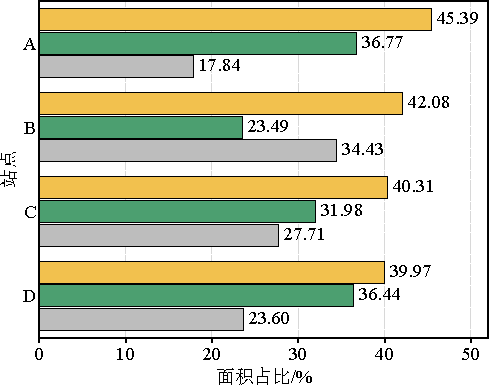
\includegraphics{study_area/fig_sec13_composition.pdf}
\par\nointerlineskip\vspace{3pt}
\classlegend
\caption{四个研究站点2023年地物面积占比}
\label{fig:sec13_composition}
\end{figure}

\subsubsection{景观格局}

本文采用FRAGSTATS计算完整参考斑块的面积（AREA）和形状指数（SHAPE）\citep{mcgarigal2023fragstats}。在各站2023年参考标签上，以8邻域相连的同类像元构成一个参考斑块。AREA表示斑块面积，SHAPE反映斑块边界相对于同面积紧凑形状的复杂程度。为避免大量微小斑块掩盖主要作物面积所在的斑块特征，分别按斑块等权和参考像元面积加权统计两项指标的分布；前者描述单个斑块的常见情况，后者描述随机取一个作物参考像元时其所在斑块的特征。

如表\ref{tab:sec13_patch_distribution}所示，按斑块等权统计，8组作物斑块的AREA中位数均仅为0.09～0.18~ha，SHAPE中位数均为1.00，反映出完整标签中存在大量细小且规则的斑块。按参考像元面积加权后，AREA中位数升至63.27～130.95~ha，说明主要作物面积集中在较大斑块中。C站玉米和大豆的面积加权SHAPE中位数分别为2.07和1.91，高于其余站点；A站分别为1.63和1.58。B站大豆的面积加权AREA中位数为63.27~ha，是8组中最低。两种权重下的数值差异表明，比较研究区斑块格局时需要同时考虑斑块数量和其承载的作物面积。

\begin{table*}[tbp]
\centering
\caption{四个研究站点2023年玉米和大豆完整参考斑块的AREA与SHAPE分布}
\label{tab:sec13_patch_distribution}
\begingroup
\songti\zihao{-5}
\setlength{\tabcolsep}{2pt}
\renewcommand{\arraystretch}{1.08}
\begin{tabular*}{\textwidth}{@{\extracolsep{\fill}}ccccccc@{}}
\toprule
\multirow{2}{*}{站点} & \multirow{2}{*}{地物类型} & \multirow{2}{*}{斑块数} & \multicolumn{2}{c}{AREA/ha} & \multicolumn{2}{c}{SHAPE} \\
\cmidrule(lr){4-5}\cmidrule(l){6-7}
 & & & 斑块等权 & 面积加权 & 斑块等权 & 面积加权 \\
\midrule
\csname @@input\endcsname tables/sec13_patch_distribution_rows.tex
\bottomrule
\end{tabular*}
\par\nointerlineskip\vspace{3pt}
\raggedright 注：数值为中位数（Q25～Q75）；面积加权以斑块包含的参考像元数为权重；SHAPE无量纲。
\par
\endgroup
\end{table*}
